\documentclass[compress]{beamer}
\usepackage{ifthen,verbatim}

\newcommand{\isnote}{}
\xdefinecolor{lightyellow}{rgb}{1.,1.,0.25}
\xdefinecolor{darkblue}{rgb}{0.1,0.1,0.7}

%% Uncomment this to get annotations
%% \def\notes{\addtocounter{page}{-1}
%%            \renewcommand{\isnote}{*}
%% 	   \beamertemplateshadingbackground{lightyellow}{white}
%%            \begin{frame}
%%            \frametitle{Notes for the previous page (page \insertpagenumber)}
%%            \itemize}
%% \def\endnotes{\enditemize
%% 	      \end{frame}
%%               \beamertemplateshadingbackground{white}{white}
%%               \renewcommand{\isnote}{}}

%% Uncomment this to not get annotations
\def\notes{\comment}
\def\endnotes{\endcomment}

\setbeamertemplate{navigation symbols}{}
\setbeamertemplate{headline}{\mbox{ } \hfill
\begin{minipage}{5.5 cm}
\vspace{-0.75 cm} \small
\end{minipage} \hfill
\begin{minipage}{4.5 cm}
\vspace{-0.75 cm} \small
\begin{flushright}
\ifthenelse{\equal{\insertpagenumber}{1}}{}{Jim Pivarski \hspace{0.2 cm} \insertpagenumber\isnote/\pageref{numpages}}
\end{flushright}
\end{minipage}\mbox{\hspace{0.2 cm}}\includegraphics[height=1 cm]{../cmslogo} \hspace{0.1 cm} \includegraphics[height=1 cm]{../tamulogo} \hspace{0.01 cm} \vspace{-1.05 cm}}

\begin{document}
\begin{frame}
\vfill
\begin{center}
\textcolor{darkblue}{\Large Beam-Halo Alignment Status Update}

\vfill
\begin{columns}
\column{0.3\linewidth}
\begin{center}
\large
\textcolor{darkblue}{Jim Pivarski}
\end{center}
\end{columns}

\begin{columns}
\column{0.3\linewidth}
\begin{center}
\scriptsize
{\it Texas A\&M University}
\end{center}
\end{columns}

\vfill
 5 May, 2010

\end{center}
\end{frame}

%% \begin{notes}
%% \item This is the annotated version of my talk.
%% \item If you want the version that I am presenting, download the one
%% labeled ``slides'' on Indico (or just ignore these yellow pages).
%% \item The annotated version is provided for extra detail and a written
%% record of comments that I intend to make orally.
%% \item Yellow notes refer to the content on the {\it previous} page.
%% \item All other slides are identical for the two versions.
%% \end{notes}

\small

\begin{frame}
\frametitle{What this talk is about}
\begin{itemize}\setlength{\itemsep}{0.75 cm}
\item Aligning incomplete rings

\item Oleg's correction to the closure problem

\item The big picture: alignment for ICHEP data
\end{itemize}
%% \hspace{-0.83 cm} \textcolor{darkblue}{\Large Outline2}
\end{frame}

%% \section*{First section}
%% \begin{frame}
%% \begin{center}
%% \Huge \textcolor{blue}{First section}
%% \end{center}
%% \end{frame}

\begin{frame}
\frametitle{Aligning incomplete rings}

\begin{itemize}
\item CSC-Overlaps alignment procedure considered so far is a solution of equations relating neighboring chambers (chamber $i$ and $i+1$)
\item Requires complete rings to be a well-defined system of equations
\item We have seen that photogrammetry still describes chamber positions well in $r\phi$: want to combine on an equal footing
\item<2> Extension of method to equations relating arbitrary $i$ and $j$:

\begin{center}
\uncover<2>{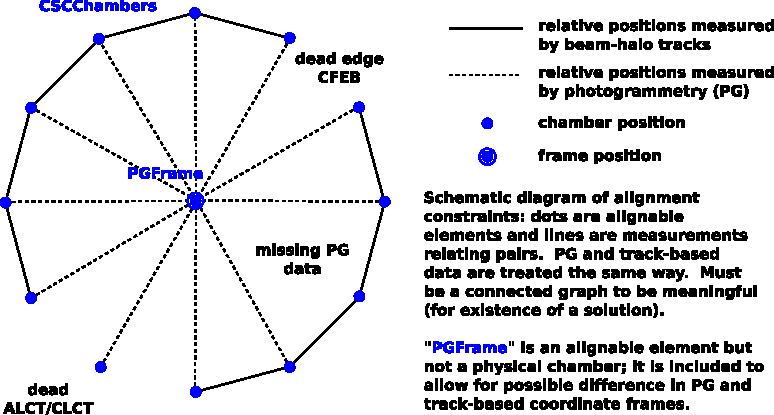
\includegraphics[width=0.9\linewidth]{beamhalo-PG.pdf}}
\end{center}
\end{itemize}
\end{frame}

\begin{frame}
\frametitle{Status}
\begin{itemize}\setlength{\itemsep}{0.25 cm}
\item Major re-write of beam-halo alignment software completed
\begin{itemize}
\item 16 new files, 2500 lines, 1.5 months
\end{itemize}
\item All of the pieces tested independently and in-situ (especially checking signs and response to test-misalignments)
\begin{itemize}
\item works in small-scale MC tests
\end{itemize}
\item Currently back to having a complete push-button procedure and
  testing with the 2010 beam-halo dataset
\end{itemize}

\vfill
\begin{itemize}\setlength{\itemsep}{0.25 cm}
\item Goal: provide combined beam-halo/photogrammetry alignment for ICHEP sign-off next week
\end{itemize}
\end{frame}

\begin{frame}
\frametitle{Oleg's closure correction}

\begin{itemize}
\item Closure per chamber = $\displaystyle \frac{1}{N} \sum_i^{N} \Delta (r\phi)_i - \Delta (r\phi)_{i+1}$ \hfill $N=18$ or $36$

\begin{itemize}
\item should be zero for complete rings, independent of $r\phi$ alignment
\item zero in 2008 $\vec{B}=0$ run, but not in 2010
\item equivalent to a change in chamber width or ring radius
\end{itemize}

\item Oleg's idea: disk bending introduces a change in radius because
  $z$ of chamber centers are not in the disks
\begin{itemize}
\item predicted that this should account for half of the effect
\item<2> it does (in old framework (below) and new framework)
\end{itemize}
\end{itemize}

\begin{center}
\only<1>{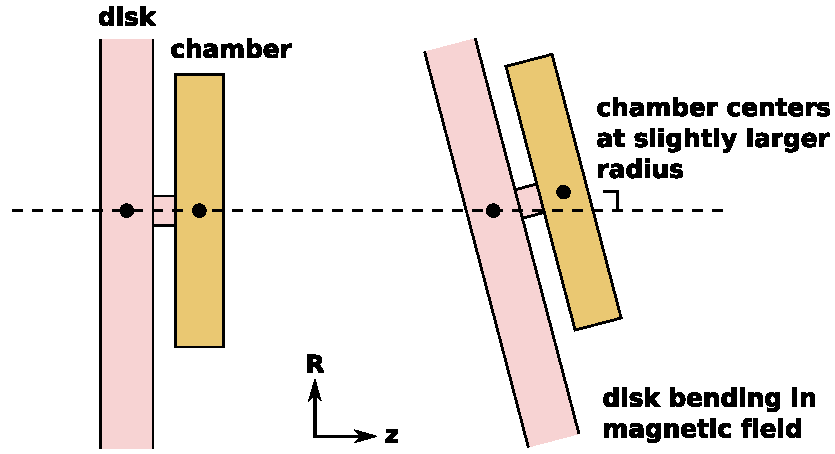
\includegraphics[width=0.6\linewidth]{olegs_correction.pdf}}
\only<2>{\begin{tabular}{c c c c}
\hline\hline
& 2008 (no $\vec{B}$) & 2010 (full $\vec{B}$) & corrected 2010 \\\hline
ME$+$3/1 &                       & $+$298 & $+$100 $\pm$ 9~$\mu$m \\
ME$-$2/1 & $-$40 $\pm$ 23~$\mu$m & & \\
ME$-$3/1 & $-$20 $\pm$ 28~$\mu$m & $+$486 & $+$278 $\pm$ 9~$\mu$m \\
ME$-$3/2 &                       & $+$572 & $+$446 $\pm$ 27~$\mu$m \\
ME$-$4/1 &                       & $+$440 & $+$267 $\pm$ 10~$\mu$m  \\\hline\hline
\end{tabular}}
\end{center}
\end{frame}

\begin{frame}
\frametitle{Big picture {\large (for track-based alignment)}}
\begin{itemize}\setlength{\itemsep}{0.25 cm}
\item Endcap alignment:
\begin{itemize}
\item chambers relative to one another: beam-halo plus photogrammetry (this talk)
\item aligned rings relative to tracker: globalMuons from 2010 cosmics; Vadim Khotilovich is implementing it as an official script based on the CRAFT-09 method
\end{itemize}

\item Barrel alignment:
\begin{itemize}
\item chambers relative to tracker: globalMuons from 2010 cosmics, using same method as CRAFT-09
\item performed by Aysen Tatarinov (with his improvements)
\item rigorous uncertainties for selecting best chambers to align
\end{itemize}

\item ICHEP reprocessing schedule:
\begin{itemize}
\item final muon alignment PVT sign-off: May 14
\item final GlobalTag: May 19
\item reprocessing of all collisions data starts late May
\item all summer 7~TeV results would be based on this
\end{itemize}
\end{itemize}
\label{numpages}
\end{frame}

\end{document}
